\section{Functions}

\begin{center}
    In this section $X$, $Y$, $U$, and $V$ are arbitrary sets.
\end{center}

A \tbf{function}\index{function} or \tbf{map}\index{function!map} $f$ from $X$ to $Y$ is a rule which, $\forall x \in X$, specifies \emph{exactly} one element of $Y$ written as
$$
f : X \to Y \qquad \text{to} \qquad X \to Y, \quad x \mapsto f(x),
$$
Here $f(x) \in Y$ is the \textbf{value}\index{function!value} of $f$ at $x$. The set $X$ is called the \tbf{domain}\index{function!domain} of $f$ and is denoted $\text{dom}(f)$ and $Y$ is the \tbf{codomain}\index{function!codomain} of $f$. Finally
$$
\text{im}(f) := \{y \in Y: \exists x \in X : y = f(x)\}
$$
is called the \tbf{image}\index{function!image} or \tbf{range}\index{function!range} of $f$, it is the subset of the codomain that is `reachable' by the function.

If $f : X \to Y$ then
$$
\text{graph}(f) := \{(x,y) \in X \times Y : y = f(x)\} = \{(x,f(x) \in X \times Y: x \in X)\}
$$
is called the \tbf{graph}\index{function!graph} of $f$.

\begin{remark}
    Let $G \setin X \times Y$ with the property $\forall x \in X, \exists! y \in Y$ with $(x,y) \in G$. The function $f : X \to Y$ with the rule that $\forall x \in X, f(x) := y, y \in Y$ where $y$ is the unique element such that $(x,y) \in G$. Clearly, $\text{graph}(f) = G$. So a function, $f:X\to Y$ is defined as the ordered triple $f = (X,G,Y), G \setin X \times Y$ such that $\forall x \in X, \exists! y \in Y, (x,y) \in G$.
\end{remark}

\subsection{Simple Examples}

$X = \vno$ and $Y = \vno$ are not excluded. If $X = \vno$ then there is only one function called the \tbf{empty function}\index{function!empty function}, $\vno : \vno \to Y$. If $Y = \vno$ but $X \neq \vno$ then there are no functions from $X$ to $Y$. Two functions $f : X \to Y$ and $g : U \to V$ are \tbf{equal}\index{function!equal}, $f = g$, if
$$
X = U, \quad Y = V\quad \text{ and } \quad f(x) = g(x), \quad \forall x \in X
$$

\begin{example}
    \begin{enumerate}[label=(\alph*)]
        \item $\text{id}_X: X \to X, x \mapsto x$ is the \tbf{identity function}\index{function!identity function} (of $X$). Sometimes written $\text{id}$ if $X$ is clear from context.

        \item If $X \setin Y$, then $i : X \to Y, x \mapsto x$ is called the \tbf{inclusion (embedding, injection)}\index{function!inclusion} of $X$ into $Y$. (sends each element of $X$ to itself while the image is viewed as an element of $Y$). Note that $i = \text{id}_X \iff X = Y$.

        \item If $X$ and $Y$ nonempty and $b \in Y$, then $f : X \to Y, x \mapsto b$ is a \tbf{constant function}\index{function!constant function}.

        \item if $f : X \to Y$ and $A \setin X$, then $f|A : A \to Y, x \mapsto f(x)$ is the \tbf{restriction of $f$ to $A$}\index{function!restriction}. Also, $f|A = f \iff A = X$.

        \item Let $A \setin X$ and $g: A \to Y$. Then any function $f : X \to Y$ with $f|A = g$ is called an \tbf{extension of $g$}\index{function!extension}, $f \supin g$.

        \item Let $f : X \to Y$ with $\text{im}(f) \setin U \setin Y \setin V$, then there are `\textbf{induced}\index{function!induced function}' functions $f_1 : X \to U$ and $f_2 : X \to V$ defined by $f_j(x) := f(x)$ for $x \in X$ and $j = 1,2$ using the same symbol for the function as needed because they are the same function just different codomains.

        \item Let $X \neq \vno$ and $A \setin X$, then the \textbf{characteristic function}\index{function!characteristic function} of $A$ is
            $$
            \chi_A : X \to \{0,1\}, \quad x \mapsto
            \begin{cases}
                1,\quad x \in A,\\
                0,\quad x \in A^c.
            \end{cases}
            $$

        \item If $X_1,\dots,X_n$ are nonempty, then projections
            $$
            \text{pr}_k : \left(\prod_{j=1}^n X_j\right) \to X_k, \quad x = (x_1,\dots,x_n) \mapsto x_k, \quad k = 1,\dots,n
            $$
            are functions.
    \end{enumerate}
\end{example}

\subsection{Composition of Functions}

Let $f : X \to Y$ and $g : Y \to V$ be two functions. Then $g \circ f$ is the \textbf{composition}\index{function!composition} of $f$ and $g$ (`$f$ followed by $g$') and is defined as
$$
g \circ f : X \to V,\quad x \mapsto g(f(x))
$$

\begin{proposition} Let $f : X \to Y$ and $g : Y \to $ and $h : U \to V$. Then $(h \circ g) \circ f$ and $h \circ (g \circ f): X \to V$ are well defined and
    \begin{equation}
        (h \circ g) \circ f = h \circ (g \circ f)
    \end{equation}
    (associativity of composition).

    \begin{proof}
        Follows directly from the definition.
        \begin{align*}
            ((h \circ g) \circ f)(x) &= (h \circ g)(f(x)) = h(g(f(x))), \\
            (h \circ (g \circ f))(x) &= h((g \circ f)(x)) = h(g(f(x))).
        \end{align*}
    \end{proof}

    \noindent Thus parenthesis are not required.
\end{proposition}

\subsection{Commutative Diagrams}
Useful to represent compositions of functions in diagrams where $X \xrightarrow{f} Y$ instead of $f : X \to Y$. The \textbf{diagram}\index{function!composition!diagram}
\[
    \begin{tikzcd}
        X \arrow{r}{f} \arrow[swap]{dr}{h} & Y \arrow{d}{g} \\
        & V
    \end{tikzcd}
\]
is \textbf{commutative}\index{function!commutative} if \(h = g \circ f\).

Similarly the diagram
\[
    \begin{tikzcd}
        X \arrow{r}{f} \arrow{d}{\varphi} & Y \arrow{d}{g} \\
        U \arrow{r}{\psi} & V
    \end{tikzcd}
\]
is commutative if \(g \circ f = \psi\circ \varphi\). Such diagrams are commutative if \(X\) and \(Y\) are sets in the diagram and on can get from \(X\) to \(Y\) via two different paths following the arrows, for example
\[
    X \xrightarrow{f_1} A_1 \xrightarrow{f_2} A_2 \xrightarrow{f_3} \cdots \xrightarrow{f_n} Y \quad \text{and} \quad X \xrightarrow{g_1} B_1 \xrightarrow{g_2} B_2 \xrightarrow{g_3} \cdots \xrightarrow{g_n} Y,
\]
then \(f_n \circ f_{n-1} \circ \cdots \circ f_1 \text{ and } g_m \circ g_{m-1} \circ \cdots \circ g_1\) are equal. The diagram
\[
    \begin{tikzcd}
        X \arrow[dd, "j"']
        \arrow[rr, "f"]
        \arrow[rrdd, near end,"\varphi", bend right=0, shift left=0, crossing over]
        & &
        Y \arrow[lldd, "\psi"', bend left=0, shift right=0, crossing over, near end]
        \arrow[dd, "g"]
        \\
        & &
        \\
        V
        & &
        U \arrow[ll, "h",shift left=0]
    \end{tikzcd}
\]
is commutative if \(\varphi = g \circ f\), \(\psi = h \circ g\), \(j = h \circ g \circ f = h \circ \varphi = \psi \circ f\) via associativity.

\subsection{Injections, Surjections, and Bijections}
Let \(f : X \to Y\) be a function. Then \(f\) is \textbf{surjective}\index{function!surjective} if \(\text{im}(f) = Y\), \textbf{injective}\index{function!injective} if \(f(x) = f(y) \implies x = y \forall x,y \in X\), and \textbf{bijective}\index{function!bijective} if \(f\) is both injective and surjective. The expressions `onto' and `one-to-one' often used to mean `surjective' and `injective' respectively. (Note: surjective intuitively means the image and the codomain are the same (the function maps to all points in the codomain), and injective intuitively means that each input maps to different outputs, i.e. each output comes from at most one input.)

\begin{example}
    \begin{enumerate}[label=(\alph*)]
        \item These images illustrate these function properties:
            \begin{center}
                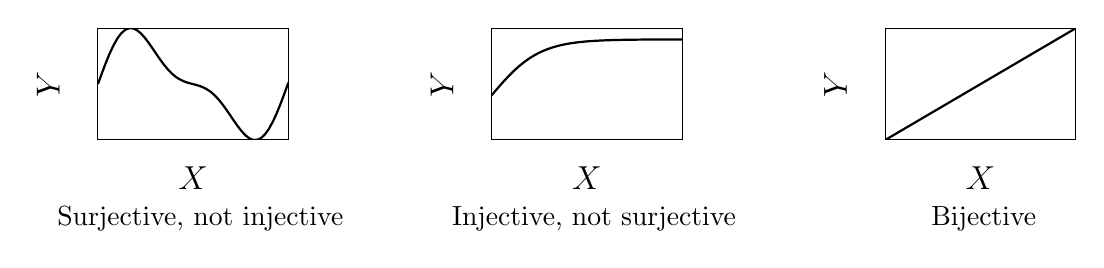
\begin{tikzpicture}

    % Surjective, not injective
    \begin{axis}[
            xshift=0cm,
            width=4cm, height=3cm,
            axis x line=box, axis y line=box,
            xtick=\empty, ytick=\empty,
            xlabel={$X$}, ylabel={$Y$},
            xlabel style={at={(0.5,-0.15)}, font=\large},
            ylabel style={at={(-0.15,0.5)}, font=\large},
            enlargelimits=false,
            % clip=true,
        ]
        \addplot[domain=0:6.3, samples=50, thick] {sin(deg(x))*0.6 + sin(deg(2*x))/4 + 1.1};
    \end{axis}
    \node at (1.3,-1.0) {Surjective, not injective};

    % Injective, not surjective
    \begin{axis}[
            xshift=5cm,
            width=4cm, height=3cm,
            axis x line=box, axis y line=box,
            xtick=\empty, ytick=\empty,
            xlabel={$X$}, ylabel={$Y$},
            xlabel style={at={(0.5,-0.15)}, font=\large},
            ylabel style={at={(-0.15,0.5)}, font=\large},
            enlargelimits=false,
            xmin=0, xmax=2,
            ymin=0, ymax=2,
        ]
        \addplot[domain=0:2, range=0:2, samples=50, thick] {tanh(2*x)+0.8};
    \end{axis}
    \node at (6.3,-1.0) {Injective, not surjective};

    % Bijective
    \begin{axis}[
            xshift=10cm,
            width=4cm, height=3cm,
            axis x line=box, axis y line=box,
            xtick=\empty, ytick=\empty,
            xlabel={$X$}, ylabel={$Y$},
            xlabel style={at={(0.5,-0.15)}, font=\large},
            ylabel style={at={(-0.15,0.5)}, font=\large},
            enlargelimits=false,
        ]
        \addplot[domain=0:2, samples=100, thick] {x+0.3};
    \end{axis}
    \node at (11.25,-1.0) {Bijective};

\end{tikzpicture}

            \end{center}

        \item Let $X_1,\dots, X_n$ be nonempty. then $\forall k \in \{1,\dots,n\}$ the $k^\text{kth}$ projection $\text{pr}_k : \prod_{j=1}^n X_j \to X_k$ is surjective, but not injective generally.
    \end{enumerate}
\end{example}

\begin{proposition}
    Let $f: X \to Y$ be a function, then $f$ is bijective if and only if there is a function $g : Y \to X$ such that $g \circ f = \text{id}_X$ and \(f \circ g = \text{id}_Y\). In this case, \(g\) is uniquely determined by \(f\), i.e. there is only one function that satisfies these properties.

    \begin{proof} Statement \(A\) is `$f$ is bijective'. Statement \(B\) is `there is a function \(g\) such that $g \circ f = \text{id}_X$ and \(f \circ g = \text{id}_Y\)'. The compound statement is \(A \iff B\).
        \begin{enumerate}[label=(\roman*)]
            \item `\(\implies\)': suppose that \(f: X \to Y\) is bijective then \(\forall y \in Y, \, \exists x \in X \st y = f(x)\) (surjective) and \(x\) is uniquely determined by \(y\), there is, at most, one \(y\) for each \(x\) (injective), together there is exactly one \(x \in X\) for every \(y \in Y\) (bijective). This defines a function \(g : Y \to X\) with the desired properties: We define a function \(g: Y \to X\) such that there is exactly one \(x \in X\) with \(f(x) = y\), so for each \(y \in Y\) define \(g(y) = x\). 
            
            Now we verify that \(g \circ f = \id_X\). Let \(x \in X\) be arbitrary, we know that \(g \circ f = g(f(x))\) by definition of a composite function. By the definition of \(g\), \(g(f(x)) = x\) and is unique thus \(g \circ f = \id_X\).

            \item `\(\Longleftarrow\)':
            
            \item
        \end{enumerate}
    \end{proof}
\end{proposition}


\subsection{Inverse Functions}

\subsection{Set Valued Functions}

\subsection*{Exercises}
